\chapter{Složitost}
\label{slozitost}

V této kapitole ukážeme několik výsledků ohledně časové a prostorové složitosti.
Problém klastrové rovinnosti patří do třídy NP z pohledu časové složitosti a z hlediska prostorového se dá řešit v prostoru $\mathcal{O}(n)$ na deterministickém stroji, kde $n$ je počet vrcholů.

Jako výchozí model uvažujeme RAM s logaritmickou velikostí paměťových buněk vzhledem k velikosti vstupu a jednotkovou cenou za aritmetické operace s čísly, případně jeho nedeterministickou verzi nRAM. Tedy polynomiálně velká čísla lze uložit a operovat s nimi v konstantním prostoru a čase. Je to standardní model u tohoto typu problémů, díky němuž lze říci, že graf s $n$ vrcholy a $m$ hranami je uložen v prostoru $\mathcal O (n+m)$.

\section{Datová reprezentace}
Nejprve uvedeme možnosti reprezentace klastrového grafu a ujasníme vzhledem k čemu budeme vztahovat příslušnou složitost. 
Pro reprezentaci klastrové hierarchie se nabízí dvě možnosti.

\begin{enumerate}
\item Seznamy vrcholů
\item Strom, kde listy představují vrcholy a vnitřní uzly představují klastry
\begin{itemize}
\item Zde předpokládejme, že kořen tohoto stromu reprezentuje klastr obsahující všechny vrcholy a listy přísluší vrcholům
\end{itemize}
\end{enumerate}

V této kapitole budeme několikrát hovořit o maximálních podklastrech (vzhledem na inkluzi) v nějakém klastru $K$. Proto si zavedeme následující definici.
\begin{defn}
Pod \textit{maximálním podklastrem vzhledem ke klastru $K$} myslíme klastr takový, že je přímým potomkem $K$ v klastrové hierarchii.
\end{defn}

Nejprve musíme určit, kolik klastrů se v klastrové hierarchii může nacházet.
Pro zjednodušení budeme předpokládat, že v klastrové hierarchii máme vždy klastr obsahující všechny vrcholy a každá jednovrcholová množina je též klastrem v klastrové hierarchii.
\begin{tvr}
Maximální počet klastrů v grafu $G$ s $n$ $(n \geq 1)$ vrcholy je $2n-1$.
\end{tvr}
\begin{proof}
Důkaz indukcí podle n: \\
Základ indukce: n=1 \\
Zjevně platí. \\
Indukční předpoklad: Tvrzení platí pro $|V| < n$.\\
Indukční krok:  \\
Díky předpokladům víme, že klastr, který obsahuje aspoň dva vrcholy, má aspoň dva maximální podklastry. \\
Máme graf s $n$ vrcholy. Podle předpokladu máme klastr $K$ obsahující všechny vrcholy. Ten obsahuje $k$ vzájemně disjunktních maximálních podklastrů. Velikost $i$-tého klastru nechť je $k_i$. Každý z těchto klastrů obsahuje méně než $n$ vrcholů. Platí pro ně tedy indukční předpoklad. Máme tedy: \\
$\text{počet klastrů } \leq 1 + \sum\limits_{i=1}^k (2*k_i-1) = 1 + 2*\sum\limits_{i=1}^k k_i - k = 2n - k + 1 $\\
K maximalizování dojde pokud bude vždy $k=2$, což odpovídá situaci, kde každý klastr, který není listem, má právě dva maximální podklastry.
\end{proof}

Velikost grafu na vstupu je  $\mathcal{O}(n+m+| \mathcal C|)$, $\mathcal C$ je klastrová hierarchie a $| \mathcal C|$ je velikost její reprezentace. První varianta reprezentace klastrové hierarchie má za následek, že klastrová hierarchie zabírá prostor až $\mathcal{O}(n^2)$. Příkladem takové klastrové hierarchie je graf, kde klastry jsou postupně do sebe vnořené. První klastr obsahuje všechny vrcholy, druhý o vrchol méně, třetí o další vrchol, ... .
Druhá varianta reprezentace naproti tomu dává prostor $\mathcal{O}(n)$. Nejvíce nám tedy o časové a prostorové složitosti problému prozradí, když budeme složitost vyjadřovat vzhledem k počtu vrcholů vstupního grafu. Dostali jsme, že klastrový graf $(G,\mathcal C )$, kde $G$ je rovinný graf, lze reprezentovat v prostoru $\mathcal O (n)$.

Dále v textu budeme pracovat výhradně se stromovou reprezentací klastrové hierarchie.

\section{Časová složitost}
Hlavním výsledkem této části je lineární nedeterministický algoritmus pro klastrovou rovinnost.
\begin{tvr}
Problém rozhodnutí existence rovinného klastrového nakreslení patří do třídy NP.
\end{tvr}
\begin{proof}
Využíváme toho, že ekvivalentním problémem ke klastrové rovinnosti je existence saturátoru. Ten nám zajistí, že klastry jsou souvislé. Saturátor dostaneme jako certifikát. Vzhledem k tomu, že klastrů je polynomiálně mnoho, tak ověření saturátoru se dá provést  v polynomiálním čase (například otestováním souvislosti každého klastru zvlášt). Dále jsou algoritmy testující klastrovou rovinnost v polynomiálním čase (viz věta \ref{souv_klastry_det_alg}), pokud klastry jsou souvislé. 
\end{proof}

\begin{tvr}
Pro problém klastrové rovinnosti je nedeterministický algoritmus, jehož časová složitost je $\mathcal{O}(n)$.
\end{tvr}
\begin{proof}

Důkaz tohoto tvrzení je pouze doplněním důkazu, že klastrová rovinnost je v NP. Pro důkaz je třeba ukázat, že umíme ověřit souvislost všech klastrů v čase $\mathcal{O}(n)$, a pak že klastrová rovinnost se dá otestovat v lineárním čase pokud jsou klastry souvislé.
Druhá část viz věta \ref{souv_klastry_det_alg}.

Prosté otestování všech klastrů zvlášť na souvislost vede na algoritmus s časovou složitostí $\mathcal O(n^2)$, protože klastrů je až lineárně mnoho a jejich celková velikost je až kvadratická. Pro zlepšení půjdeme cestou, kdy budeme testovat souvislost klastrů od nejmenších k největším. A po otestování klastru na souvislost daný klastr zkontrahujeme do jediného vrcholu, abychom při testování nadklastrů nemuseli opětovně procházet přes vrcholy otestovaného klastru.

Při testování klastru na souvislost použijeme klasický algoritmus na testování souvislosti. Hrany, které vedou ven z klastru, si při průchodu si je zapamatujeme, a po doběhnutí testu je aktualizujeme, tedy nasměrujeme je do nového vrcholu vzniklého kontrakcí klastru. Časová složitost pro jeden klastr C je $\mathcal{O}(n_C + m_C + \#$počet hran ven z klastru), kde $n_C$ je počet vrcholů klastru a $m_C$ je počet hran mezi vrcholy klastru. Problémem je, že tohle stále vede na algoritmus s kvadratickou časovou složitostí (TODO obrázek klastrového klastru dosvědčující tuto složitost). Je to způsobeno tím, že se hrany můžou aktualizovat příliš často.

\begin{figure}[H]
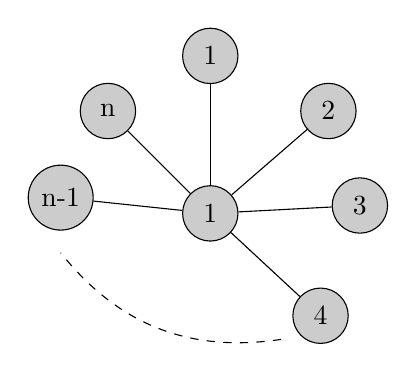
\begin{tikzpicture}[node/.style={circle,fill=black!20,draw,minimum size=2em,inner sep=3pt]}]

    \node[node] (1) at (0,0) {1};
    \node[node] (2) at (0, 2)  {1};
    \node[node] (3) at (1.5, 1.3) {2};
    \node[node] (4) at (1.9,0.1) {3};
    \node[node] (5) at (1.4, -1.3)  {4};
    \node[node] (6) at (-1.9, 0.2) {n-1};
    \node[node] (7) at (-1.3, 1.3) {n};

    \draw (1) -- (2);
    \draw (1) -- (3);
    \draw (1) -- (4);
    \draw (1) -- (5);
    \draw (1) -- (6);
    \draw (1) -- (7);
    \draw[dashed] (0.9,-1.6) to [bend left] (-1.9,-0.5);
\end{tikzpicture}
\caption{Klastrový graf, pro který poběží kvadraticky dlouho vzhledem k počtu vrcholů algoritmus s aktualizací hran. Je to hvězda, kde $i$-tý klastr je tvořen vrcholy s čísly nejvýše $i$. Důvodem neefektivity je to, že kontrakce vždy zasáhne středový vrchol hvězdy a všechny hrany se musí přesměrovat do nového vrcholu vzniklého kontrakcí.}
\end{figure}

Nyní uvedeme algoritmus s lineární časovou složitostí. Ten vychází z předchozího pokusu, kde jsme si zdánlivě nepomohli. Pro zlepšení musíme dosáhnout toho, že hrany opakovaně nenavštěvujeme. To provedeme následovně: Pro každý klastr $K$ budeme mít pomocný graf (označme jej $G_K$, kde vrcholy představují maximální podklastry daného klastru. Hrany v těchto pomocných grafech představují hrany jdoucí mezi klastry. Každé hraně $\{x,y\}$ v grafu $G$ odpovídá hrana v právě jednom pomocném grafu. Abychom mohli určit, do kterého pomocného grafu hrana patří, tak potřebujeme určit nejmenší klastr, který sdílejí vrcholy příslušné hrany. Navíc také potřebujeme znát podklastry, kam vrcholy patří. To je ale problém nejmenšího společného předka v zakořeněném stromu, kdy potřebné dotazy se provádí v konstantním čase a s lineárním předvýpočtem a využívající lineární prostor. Jednoduchou úpravou získame i ty potřebné informace (ty podklastry). (TODO přidat referenci na LCA a RMQ)

Náš algoritmus tedy napřed provede předvýpočet potřebný pro problém hledání minimální společného předka, kde se hrany rozdělí do pomocných grafů. Následně se pro každý pomocný graf provede test souvislosti. První část algoritmu pracuje v čase $\mathcal{O}(n)$ díky tomu, že umístění hrany do pomocného grafu umíme provést v konstantním čase a hran je pouze $\mathcal{O}(n)$. Druhá část algoritmu pracuje v čase $\sum\limits_{C \in \mathcal C}(n_{G_C}+m_{G_C}) = \sum\limits_{C \in \mathcal C}n_{G_C} + \sum\limits_{C \in \mathcal C}m_{G_C} \leq \text{počet klastrů} + m = \mathcal O(n) + \mathcal O(n)=\mathcal O(n)$, zde $n_{G_C}$ značí počet vrcholů pomocného grafu a $m_{G_C}$ počet jeho hran.
\end{proof}

\section{Prostorová složitost}
Z výsledků o časové složitosti můžeme říci, že můžeme klatrovou rovinnost rozhodovat v nedeterministickém prostoru o velikosti $\mathcal{O}(n)$. Ze Savitchovy věty (doplnit ref) plyne, že v deterministickém prostoru stačí nejvýše prostor velikosti $\mathcal{O}(n^2)$.
Lepšího výsledku, ve smyslu, že potřebujeme méně prostoru, dosáhneme využítím vztahu tříd NTIME a DSPACE, který je $NTIME(t(n)) \subseteq DSPACE(t(n))$. Jelikož máme nedeterministický algoritmus pro klastrovou rovinnost pracující v lineárním čase, tak díky předešlému víme, že existuje deterministický algoritmus využívající pouze lineárně mnoho prostoru.
\begin{tvr}
Klastrová rovinnost lze rozhodovat na RAMu s lineárně omezeným prostorem.
\end{tvr}
\begin{proof}
\end{proof}

% nekopírovat
2.1
\label{souv_klastry_det_alg}